% ─────────────────────────────────────────────────────────────────────────────
% RESULTS SECTION --- HyperFisher Thesis
% Assumes figures live in a /figures subfolder in Overleaf.
% ─────────────────────────────────────────────────────────────────────────────

\section{Results}
\label{sec:results}

For each sub-research question, we describe the experimental scope, present the key
quantitative findings, and highlight the most important patterns. 
Average accuracy ($A_T$) is the primary evaluation metric, and backward transfer 
($\mathrm{BWT}$) is reported as a secondary measure of forgetting. Standalone target-network 
results that establish the reference behaviour of projection methods in their original, 
non-hypernetwork setting are provided in Appendix~B (Figure~\ref{fig:standalone_trajectories_all}).

% ─────────────────────────────────────────────────────────────────────────────
\subsection{Sub-RQ1: Constructive Synergy or Architectural Conflict?}
\label{sec:results_rq1}

Three hypernetwork regimes are evaluated: a standard-capacity Split-CIFAR10 network, an extremely compressed Split-MNIST network (suffocated regime, $d_h = 8$), and a ten-task Split-CIFAR100 network.

\paragraph{Standard hypernetwork --- Split-CIFAR10.}
Figure~\ref{fig:hn_cifar10} presents average accuracy and BWT for all eight methods on Split-CIFAR10 with a standard-capacity hypernetwork and full normalization enabled.
Plain \texttt{SGD} at $84.1\%$ establishes the unconstrained reference, and \texttt{Adam} at $90.4\%$ defines the upper frontier.
\texttt{iFOPNG} leads all projection methods at $86.0\%$, the only one to surpass \texttt{SGD}.
The remaining methods fall below the \texttt{SGD} reference: \texttt{EWC} at $83.1\%$, \texttt{FNG} at $81.1\%$, \texttt{OGD} at $79.6\%$, \texttt{FOPNG} at $77.9\%$, and \texttt{ONG} at $71.4\%$.
\texttt{Adam} has effectively zero backward transfer ($\mathrm{BWT} \approx 0.000$), while all projection methods exhibit small but nonzero forgetting (\texttt{iFOPNG}: $-0.013$; \texttt{FOPNG}: $-0.015$).

\begin{figure}[H]
    \centering
    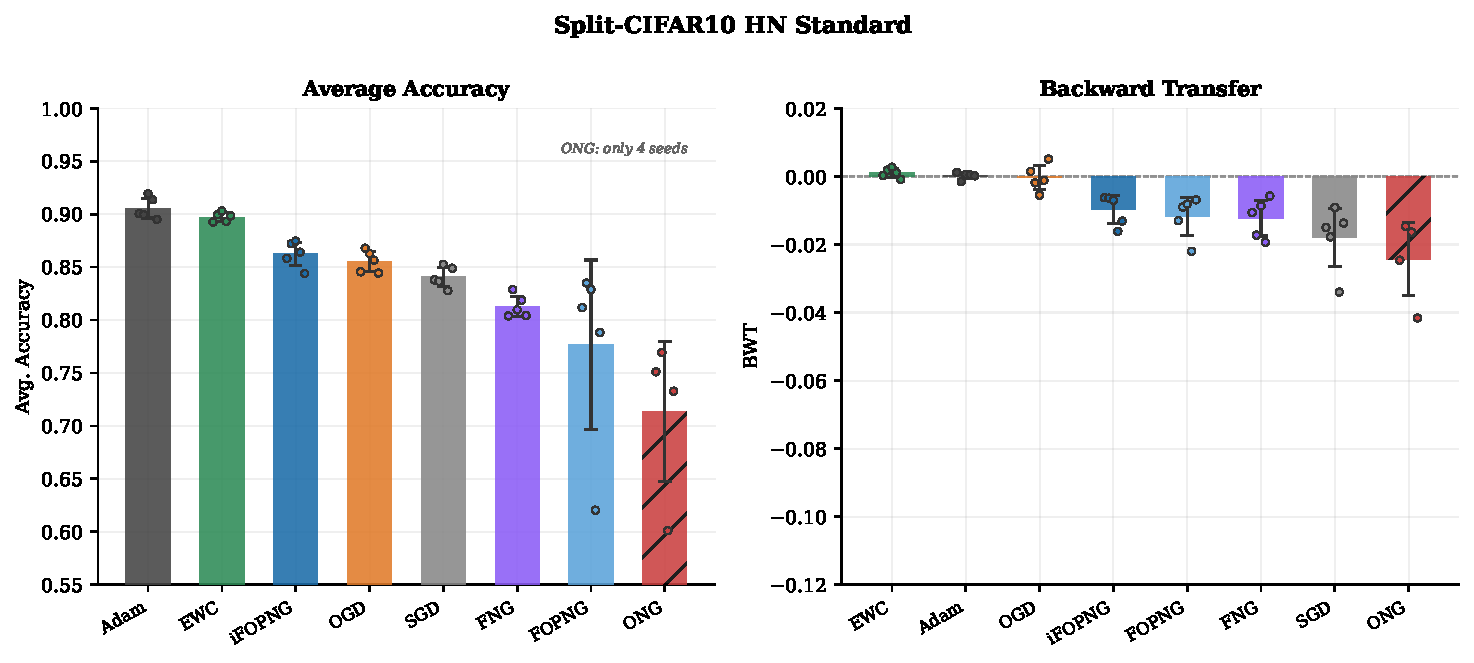
\includegraphics[width=\linewidth]{figures/hypernetwork-cifar10_8.pdf}
    \caption{%
        \textbf{Split-CIFAR10 hypernetwork (5 tasks, 50 epochs
        per task, AdamW first-task initialisation at $10^{-3}$).}
        Left: average accuracy (bars show mean over seeds; circles show
        individual seeds).
        Right: backward transfer. Methods are sorted by
        average accuracy on the left panel.
        \texttt{Adam} defines the projection-free upper frontier;
        \texttt{SGD} defines the unconstrained reference at $84.1\%$.
        \texttt{iFOPNG} is the only projection method to exceed \texttt{SGD};
        the remaining projection variants fall below it.
        All experiments use full normalization (Section~\ref{sec:results_rq2}).
    }
    \label{fig:hn_cifar10}
\end{figure}

\paragraph{Suffocated regime --- Split-MNIST, $d_h = 8$.}
Figure~\ref{fig:hn_suffocated} presents the full method comparison.
\texttt{Adam} leads at $92.7\%$.
\texttt{EWC} is the strongest regularization baseline at $87.5\%$, followed by the Fisher-free projection method \texttt{OGD} at $86.1\%$ and \texttt{SGD} at $78.4\%$.
The Fisher-based methods fall below: \texttt{iFOPNG} at $77.2\%$, \texttt{FOPNG} at $65.4\%$, and \texttt{FNG} at $63.4\%$.
Unlike previous observations, \texttt{iFOPNG}, \texttt{FOPNG}, and \texttt{FNG} all suffer from substantial negative backward transfer ($\mathrm{BWT}$ between $-0.15$ and $-0.21$), while \texttt{Adam} maintains a much smaller negative BWT ($-0.068$) and \texttt{SGD} forgets substantially ($-0.180$).

\begin{figure}[H]
    \centering
    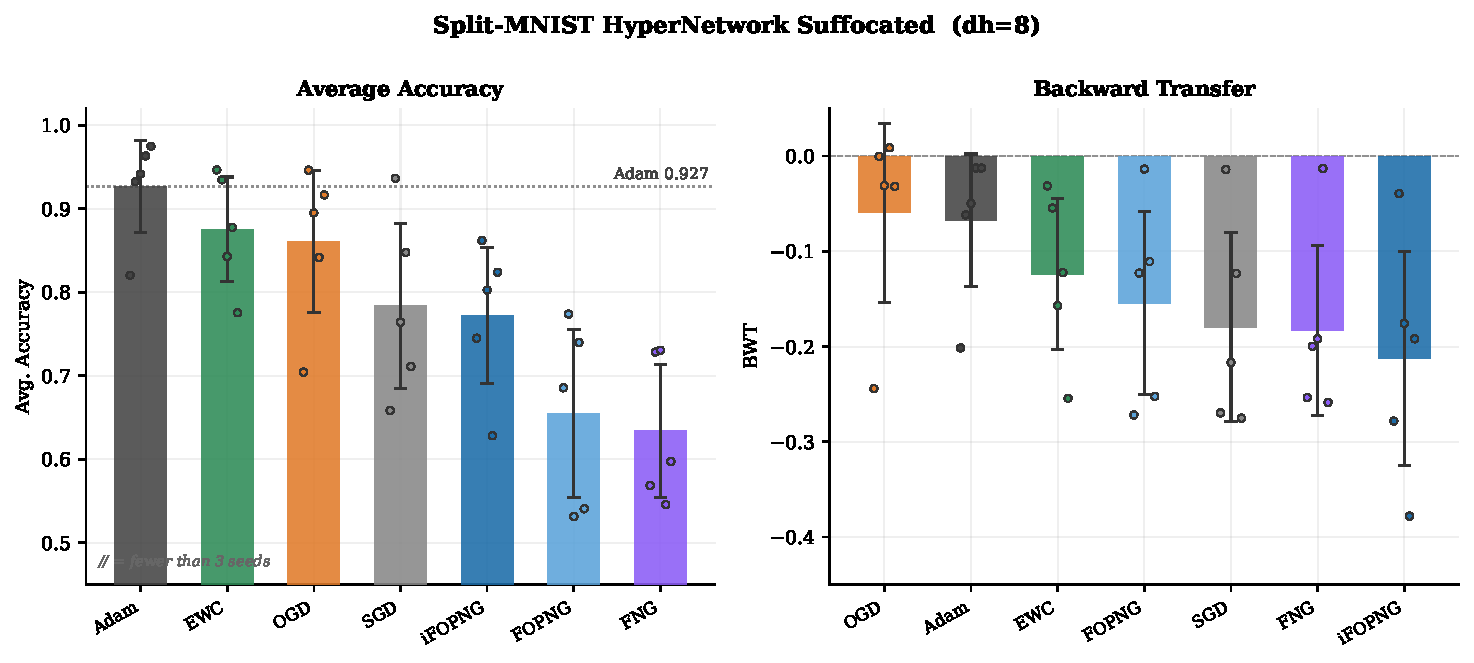
\includegraphics[width=\linewidth]{figures/hypernetwork-suffocated_7.pdf}
    \caption{%
        \textbf{Split-MNIST SH hypernetwork, suffocated
        regime ($d_h = 8$, 5 tasks, 15 epochs per task, \texttt{AdamW}
        first-task initialisation).}
        Left: average accuracy (bars show mean over seeds; circles show
        individual seeds).
        Right: backward transfer.
        The dotted line marks \texttt{Adam}'s mean accuracy ($92.7\%$).
        Fisher-based projection methods (\texttt{iFOPNG}, \texttt{FOPNG},
        \texttt{FNG}) suffer from significant negative BWT and lower accuracy than
        \texttt{Adam}, revealing a retention failure in the extreme compression regime.
        \texttt{EWC} is the best-performing baseline at $87.5\%$, while the Fisher-free \texttt{OGD} achieves $86.1\%$.
    }
    \label{fig:hn_suffocated}
\end{figure}

\paragraph{Extended task count --- Split-CIFAR100.}
At ten tasks on Split-CIFAR100 (Appendix~Figure~\ref{fig:hn_cifar100}), \texttt{EWC} unexpectedly leads at $45.5\%$, with \texttt{Adam} second at $42.0\%$ and \texttt{iFOPNG} third at $37.8\%$ (random baseline: $10.0\%$).

% ─────────────────────────────────────────────────────────────────────────────
\subsection{Sub-RQ2: Normalization Resolves the Gradient Pathology}
\label{sec:results_rq2}

This subsection reports the three-condition normalization ablation.
Figure~\ref{fig:norm_conditioning} traces the $\log_{10}$ condition number of the projection kernel $G^\top F G$ over training steps;
Figure~\ref{fig:norm_ablation} shows the resulting average accuracy and BWT under each condition.

\begin{figure}[H]
    \centering
    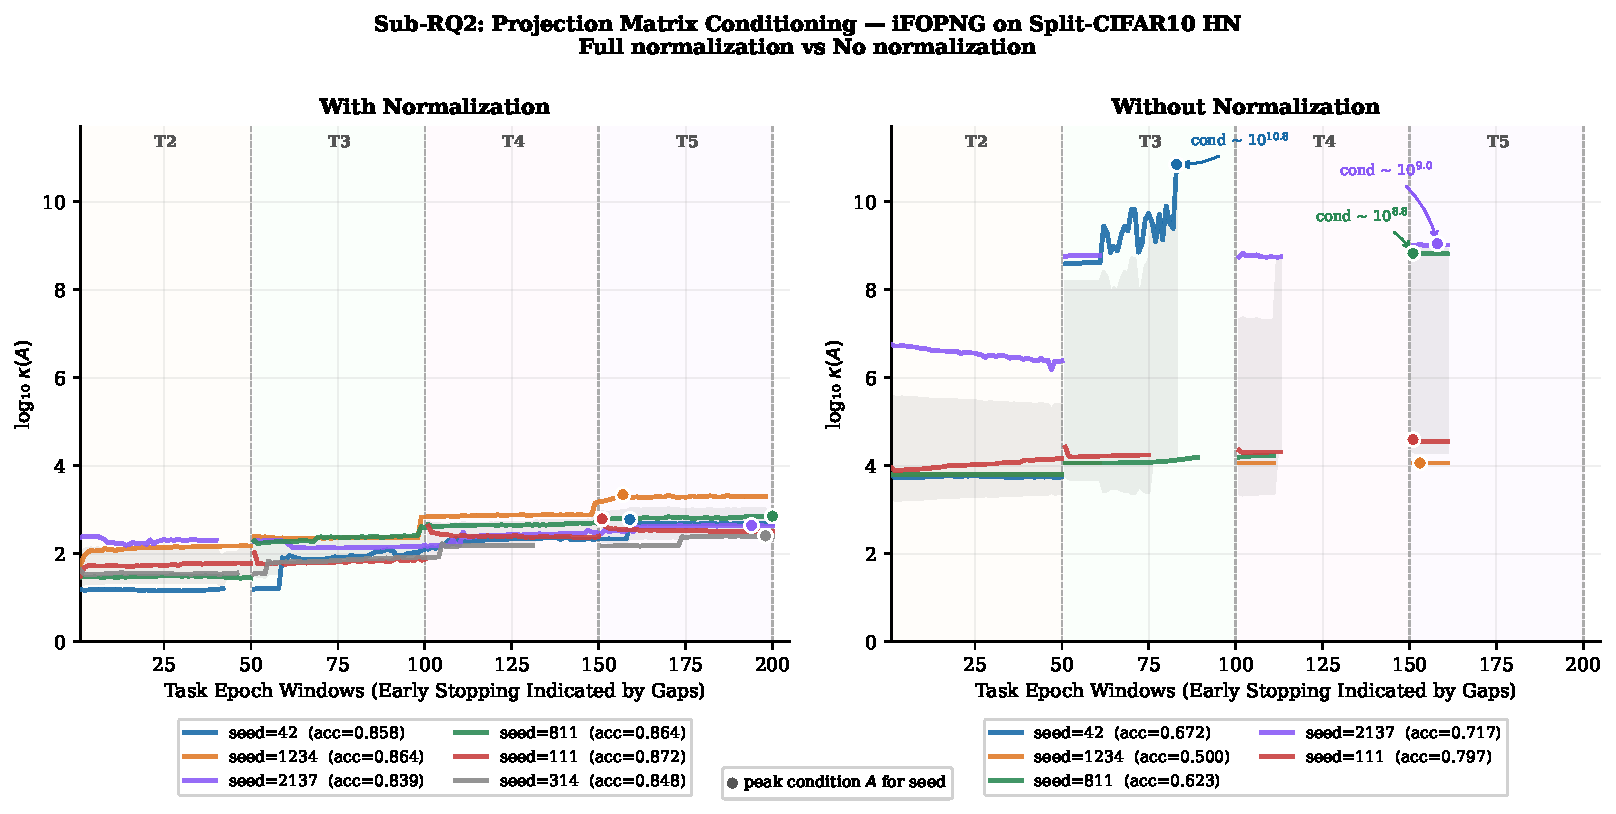
\includegraphics[width=\linewidth]{figures/normalization-conditioning_8-9.pdf}
    \caption{%
        \textbf{Projection kernel condition number over training ---
        \texttt{iFOPNG} on Split-CIFAR10 HN.}
        Each line is one seed (legend shows final average accuracy).
        Task boundaries are marked by vertical dashed lines; gaps indicate
        early stopping.
        Left (full normalization): $\log_{10}\kappa(A)$ remains bounded within $[10^{1.3},\,10^{3.3}]$ throughout.
        Right (no normalization): condition number spikes to
        $10^{10.8}$ at the T2$\to$T3 transition, causing projection failure.
        Diamond markers indicate end-of-task condition number values.
    }
    \label{fig:norm_conditioning}
\end{figure}

\begin{figure}[H]
    \centering
    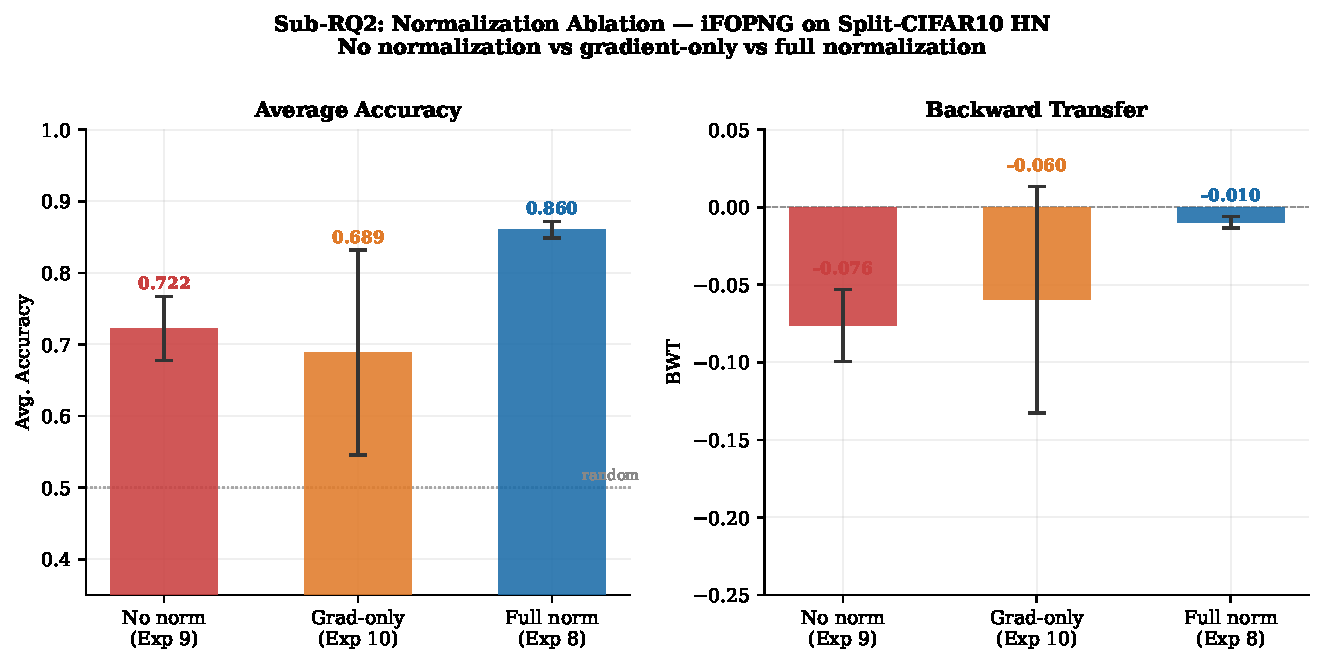
\includegraphics[width=0.75\linewidth]{figures/normalization-ablation_8-9-10.pdf} 
    \caption{%
        \textbf{Normalization ablation --- \texttt{iFOPNG} on Split-CIFAR10 HN
        (Sub-RQ2).}
        Three conditions: no normalization, gradient-only
        normalization, and full normalization.
        Left: average accuracy with mean annotated on each bar.
        Right: backward transfer.  Circles show individual seeds;
        bars show the mean.
        The dotted line on the left panel marks random-chance
        performance ($50\%$ for binary per-task classification).
    }
    \label{fig:norm_ablation}
\end{figure}

\paragraph{Without normalization.}
The right panel of Figure~\ref{fig:norm_conditioning} shows the condition number reaching $10^{10.8}$ at the T2$\to$T3 task transition for the most-affected seed, stabilizing near $10^{8.8}$--$10^{9.0}$ for two others.
The result is $72.2\%$ average accuracy and $\mathrm{BWT} = -0.076$.

\paragraph{Gradient-only normalization.}
Applying unit-$\ell_2$ column normalization to $G$ alone recovers $65.9\%$ (BWT $-0.065$), below both full normalization ($86.0\%$) and the no-normalization baseline ($72.2\%$) (Figure~\ref{fig:norm_ablation}).

\paragraph{Full normalization.}
Combining column-wise $\ell_2$ normalization of $G$ with absolute-maximum scaling of $F$ maintains $\log_{10}\kappa(A)$ bounded within $[10^{1.3},\,10^{3.3}]$ across all seeds and task transitions, a reduction of roughly seven orders of magnitude relative to the no-normalization condition (Figure~\ref{fig:norm_conditioning}).
Average accuracy recovers to $86.0\%$ and BWT improves to $-0.010$ (Figure~\ref{fig:norm_ablation}).

% ─────────────────────────────────────────────────────────────────────────────
\subsection{Sub-RQ3: Parameter Inertia via the Combined Fisher Metric}
\label{sec:results_rq3}

Figure~\ref{fig:ifopng_comparison} presents mean average accuracy for \texttt{iFOPNG} and \texttt{FOPNG} across all eight benchmarks.

\begin{figure}[H]
    \centering
    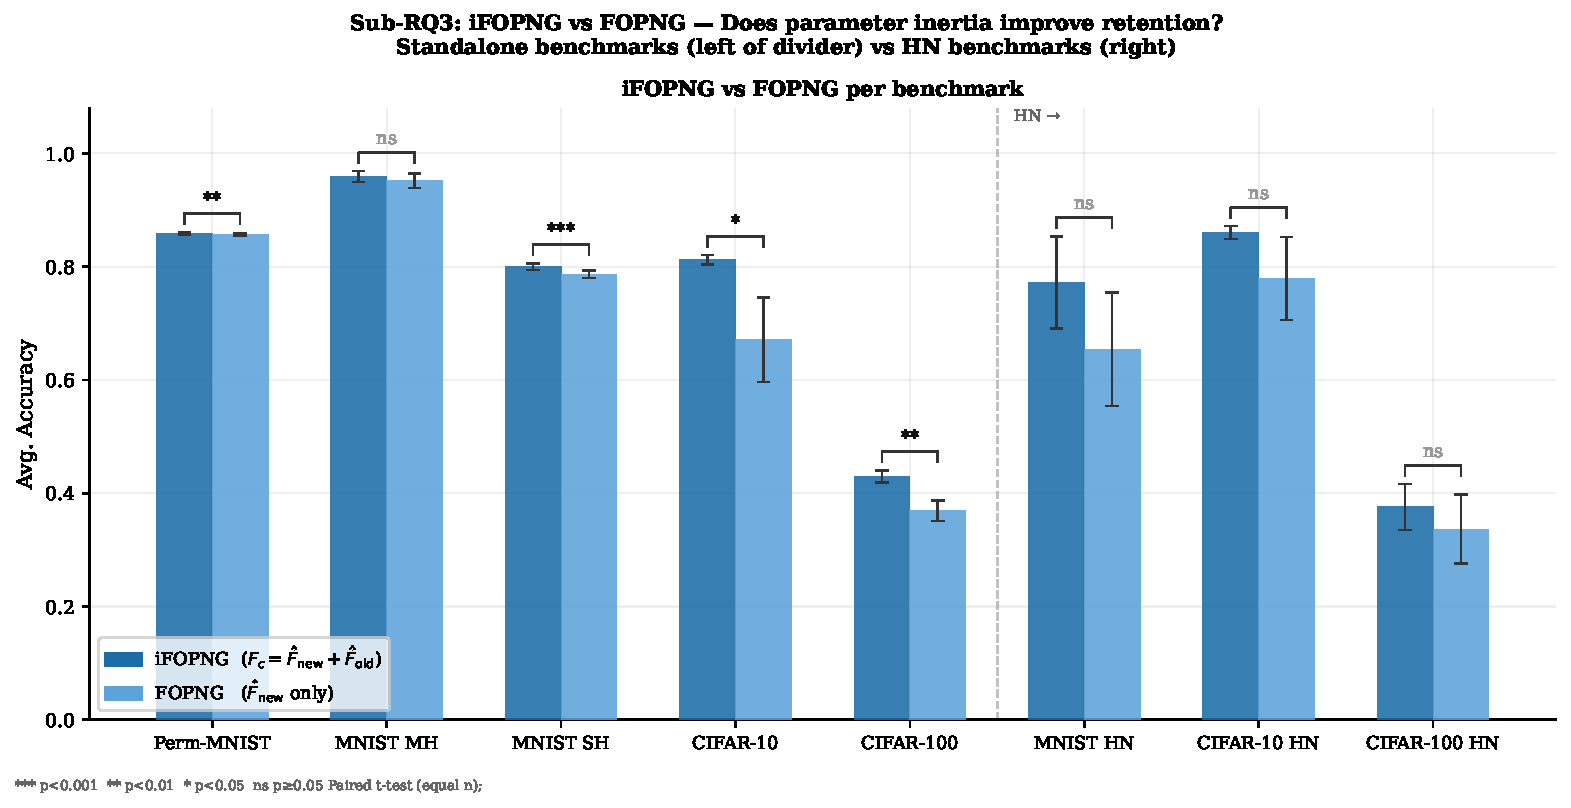
\includegraphics[width=\linewidth]{figures/projection-comparison_1-2-3-4-6-7-8.pdf}
    \caption{%
        \textbf{iFOPNG vs.\ FOPNG across eight benchmarks (Sub-RQ3).}
        Grouped bars show mean average accuracy;
        circles show individual seeds;
        error bars show $\pm 1$ standard deviation.
        The dashed vertical line
        separates standalone (left) from hypernetwork (right) settings.
        \texttt{iFOPNG} uses the combined metric
        $F_c = F_\mathrm{new} + F_\mathrm{old}$;
        \texttt{FOPNG} uses only $F_\mathrm{new}$.
    }
    \label{fig:ifopng_comparison}
\end{figure}

On the two simplest benchmarks the absolute differences are small, but the two cases 
diverge statistically. On Permuted-MNIST the $0.3$~pp advantage is negligible in size 
yet highly consistent across seeds, and reaches significance ($85.9\%$ vs.\ $85.7\%$, 
$t(4) = 6.38$, $p = .003$, $d_z = 2.85$, $n = 5$). On Split-MNIST multi-head a similarly 
small near-ceiling gap does not reach significance ($95.9\%$ vs.\ $95.2\%$, $t(4) = 1.12$, $p = .325$, $n = 5$).
% ─────────────────────────────────────────────────────────────────────────────
\subsection{Sub-RQ4: Fisher Accumulation Operator}
\label{sec:results_rq4}

This subsection compares two strategies for accumulating $F_\mathrm{old}$ across tasks under the \texttt{iFOPNG} combined Fisher metric: the element-wise maximum operator (MAX) and an exponential moving average (EMA).
Both are evaluated on a twenty-task Permuted-MNIST sequence with five random seeds.
Figure~\ref{fig:ema_trajectory} presents the average accuracy and backward transfer trajectories over all twenty tasks.

\begin{figure}[H]
    \centering
    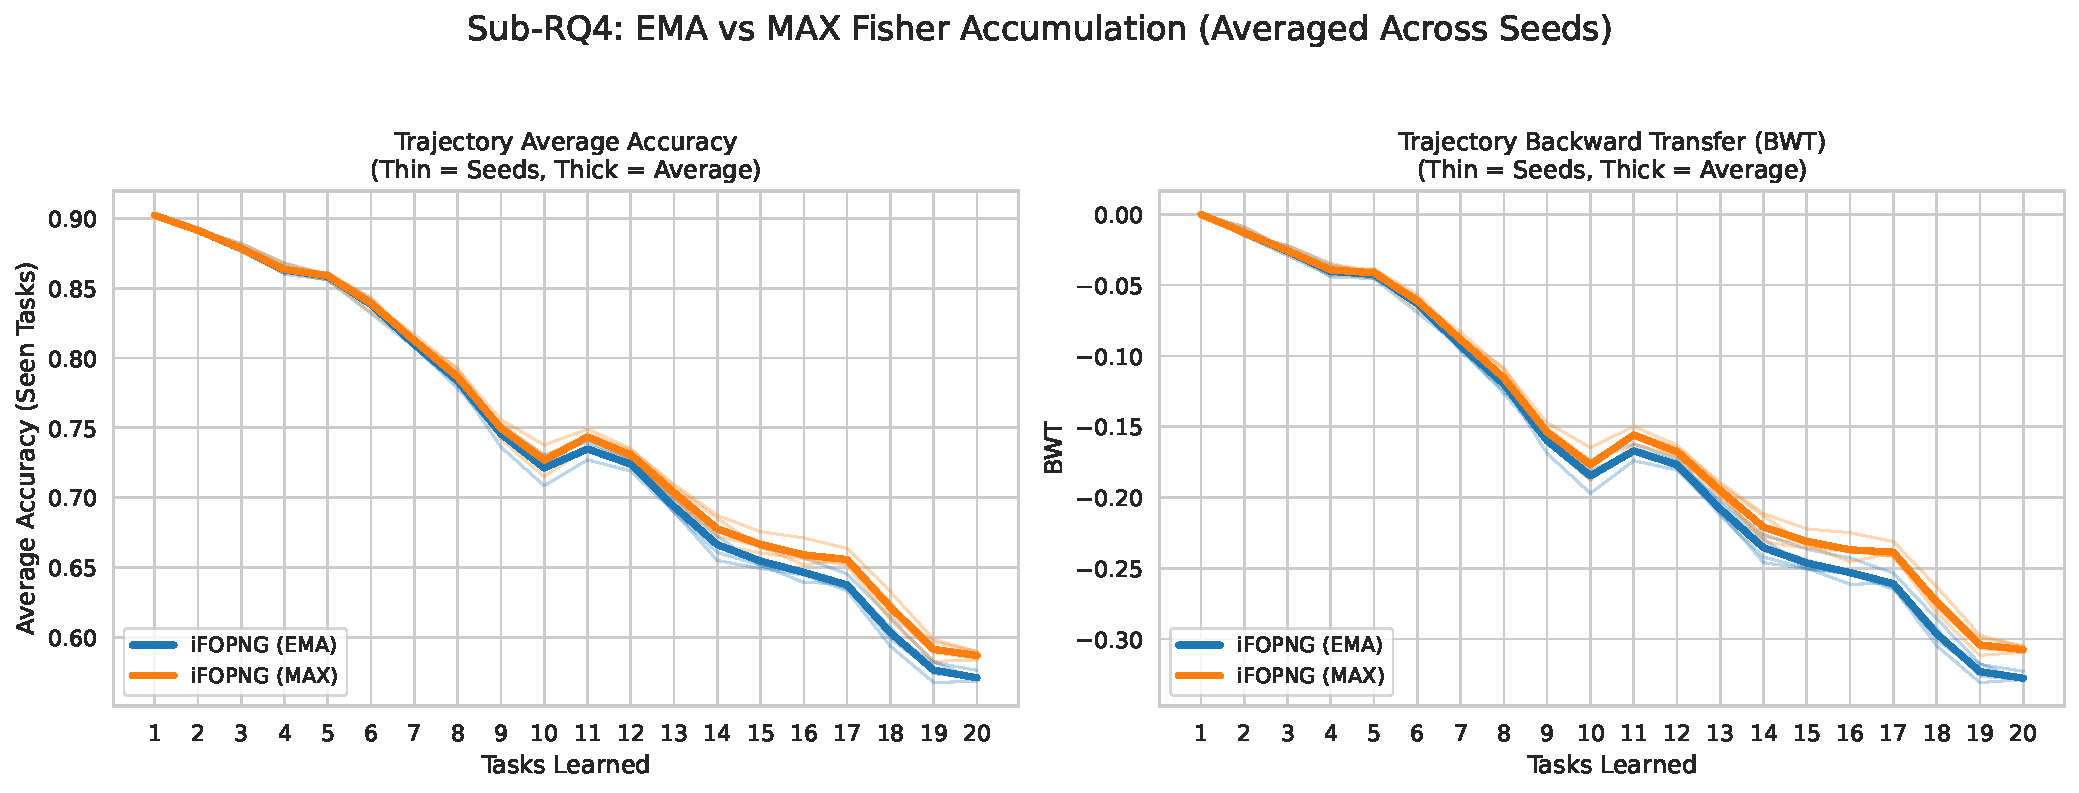
\includegraphics[width=\linewidth]{figures/ema-vs-max-trajectory_14-15.pdf}
    \caption{%
        \textbf{EMA vs.\ MAX Fisher accumulation trajectories on 20-task
        Permuted-MNIST (Sub-RQ4), $n = 5$ seeds.}
        Thick lines show the seed-averaged trajectory;
        thin lines show individual seeds.
        Left: average accuracy over tasks seen so far, evaluated after each
        task is trained.
        Right: backward transfer over the same sequence.
        MAX leads EMA by a consistent margin across all five seeds;
        both strategies produce closely tracking trajectories throughout the
        full twenty-task sequence.
    }
    \label{fig:ema_trajectory}
\end{figure}

A paired $t$-test on final average accuracy establishes MAX as the superior operator: $t(4) = 14.43$, $p < 0.001$, $d_z = 6.45$.
MAX leads EMA by $1.50$--$1.65$ percentage points across every seed pair without exception.